
\documentclass[conference]{IEEEtran}

\usepackage{graphicx}
\usepackage{enumerate}
\usepackage[numbers]{natbib}
\usepackage{url} % not crucial - just used below for the URL 
\usepackage{amsmath}
\usepackage{amsfonts}
\usepackage{amssymb}
\usepackage[all]{xy}
\usepackage{color}
\usepackage{subfig}
%\usepackage{graphicx,psfrag,epsf}
\newcommand{\fixd}[1]{\textcolor{red}{\bf #1}} %dani's color


% correct bad hyphenation here
\hyphenation{op-tical net-works semi-conduc-tor}


\begin{document}
%
% paper title
% Titles are generally capitalized except for words such as a, an, and, as,
% at, but, by, for, in, nor, of, on, or, the, to and up, which are usually
% not capitalized unless they are the first or last word of the title.
% Linebreaks \\ can be used within to get better formatting as desired.
% Do not put math or special symbols in the title.
\title{Convolutional Neural Networks for Scientific Images: Simulation and Experimental Data}


% author names and affiliations
% use a multiple column layout for up to three different
% affiliations
\author{\IEEEauthorblockN{Michael Shell}
\IEEEauthorblockA{School of Electrical and\\Computer Engineering\\
Georgia Institute of Technology\\
Atlanta, Georgia 30332--0250\\
Email: http://www.michaelshell.org/contact.html}
\and
\IEEEauthorblockN{Homer Simpson}
\IEEEauthorblockA{Twentieth Century Fox\\
Springfield, USA\\
Email: homer@thesimpsons.com}
\and
\IEEEauthorblockN{James Kirk\\ and Montgomery Scott}
\IEEEauthorblockA{Starfleet Academy\\
San Francisco, California 96678--2391\\
Telephone: (800) 555--1212\\
Fax: (888) 555--1212}}


\maketitle

% As a general rule, do not put math, special symbols or citations
% in the abstract
\begin{abstract}
What is the science question we are trying to solve
Why is it hard
Contribution

\end{abstract}

% no keywords


% For peer review papers, you can put extra information on the cover
% page as needed:
% \ifCLASSOPTIONpeerreview
% \begin{center} \bfseries EDICS Category: 3-BBND \end{center}
% \fi
%
% For peerreview papers, this IEEEtran command inserts a page break and
% creates the second title. It will be ignored for other modes.
\IEEEpeerreviewmaketitle



\section{Introduction}
% no \IEEEPARstart
Recent estimates for daily data generation are around 2.5 quintillion ($10^{18}$) bytes. As an example, the instrument upgrades at the Department of Energy (DOE) facilities, including accelerator and detector technology, are yielding an unprecedented increase in the quantity and complexity of raw data, especially in multi-domain experimental facilities, such as synchrotrons or neutron sources. The variety of equipment enables thousands of researchers to pursue investigations across a wide range of areas, from archeology and biology to physics and nano-science. While the science is diverse, the underlying image analyses required to measure fundamental quantities about the experiments, follow a
relatively smaller set of patterns. These patterns or motifs consist of statistical schemes and data formats, which when incorporated to emerging machine learning (ML) algorithms, can leverage large repositories of curated data, and enable discovery at scientifically relevant solution spaces.

Our paper will describe how space and intensity variations work as computational motifs and how to use ML algorithms to image-centric data, including numerical schemes for automated characterization of materials components. Our preliminary use-cases include records of high-resolution data, coming from scientific experiments, particularly those reliant on advanced instruments and simulations. We will address our three main research and development activities:
1) Data sources: by coupling Observational, Simulation, and User-interaction data: how to retrieve
more relevant outcomes, even when using vast amounts of multimodal experimental records;
2) Software tools: we have deployed ML algorithms using deep learning, e.g., convolutional neural
networks for conventional and heterogeneous architectures, such as the low-power consumption IBM True
North neuromorphic chip, as illustrated in Figure 1;
3) Use-cases: we have analyzed large datasets of x-ray scattering data (HipGISAXS), as in Figure 2,
running on massively parallel machines, and, more generally, analysis of image-based experiments for
quantifying material composition and structures (e.g. QuantCT/IDEAL), exploring graph-based methods.
Finally, we will discuss how these images across domains can be processed using similar tools and/or
motifs, and how higher levels of concurrency promoted by new computing systems may provide online
feedback to steer experiments and collect more information from data.


%From joao
The architecture of Convolutional Neural Networks (CNN) depend on a
large number of parameters, obtained from the data and derived weights,
found during a through search over the hyperparameter space. The
memory footprint to compute and store CNN models demand research
on methods to adapt CNN to energy efficient devices. This work focuses
on data reduction schemes and net weight representations in order to
accurately classify scientific data from simulations. Our scheme reduces
double-format values to one byte,maintaining classification accuracy
above 98\%.

\section{Related work}


\section{Simulating and recording scientific data}
History about synthesis, screening, characterization, discovery and re-discovery (retrieval)

\subsection{Cryo-EM}
chao/joao

\subsection{Scattering}
We propose a supervised classification approach to identify the crystal lattice types from a Grazing
Incidence Small Angle X-ray Scattering (GISAXS) image. GISAXS is an important reciprocal-space imaging
modality which provides statistical information about a sample in 3-D. GISAXS is widely used for
studying thin films that play a vital role as building blocks for the next generation of renewable
energy technology. One challenge in GISAXS imaging is to accurately infer the crystal lattice
corresponding to the sample from a single 2-D diffraction/scatter pattern.

As a first step towards understanding crystal configurations, we use a simulation package termed
HiPGISAXS [1], to generate a large collection of sample images from each class of possible crystal
structures and test the algorithm performance under multiple simulated test images. Inspired by the
recent success of deep-learning approaches for natural image classification, we use a Convolutional
Neural Network (CNN) [2] method to carry out the classification.

We address the problem of classifying GISAXS patterns from 7 different crystal lattices (classes). We
generated 1,000 images with dimensions of 100X100 pixels for each class by varying the lattice
parameters as input to a 4 layer CNN to train a classifier. The architecture of this network is
adapted from the MNIST classifier used by MatConvNet. We tested the performance of the classifier on
multiple data sets, including samples corrupted with realistic noise levels. We obtained an accuracy
that ranged from 82.6\% to 92.29\% depending on the parameters of each test case which we believe is
an encouraging result for further extending the use of CNNs for GISAXS as well as other synchrotron
based scientific experiments.

\subsection{Phase contrast}


\begin{figure*}[t!]
\centering
\subfloat[Case I]{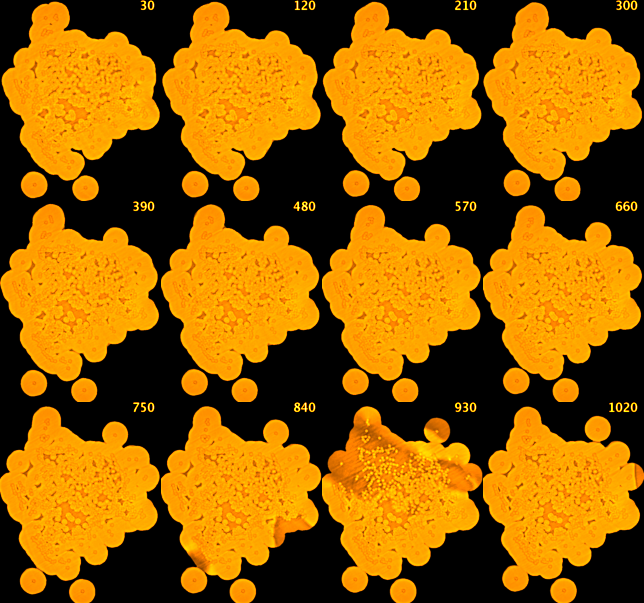
\includegraphics[width=2.5in]{img/fiberMontage.png}
\label{fig_first_case}}
\hfil
\subfloat[Case II]{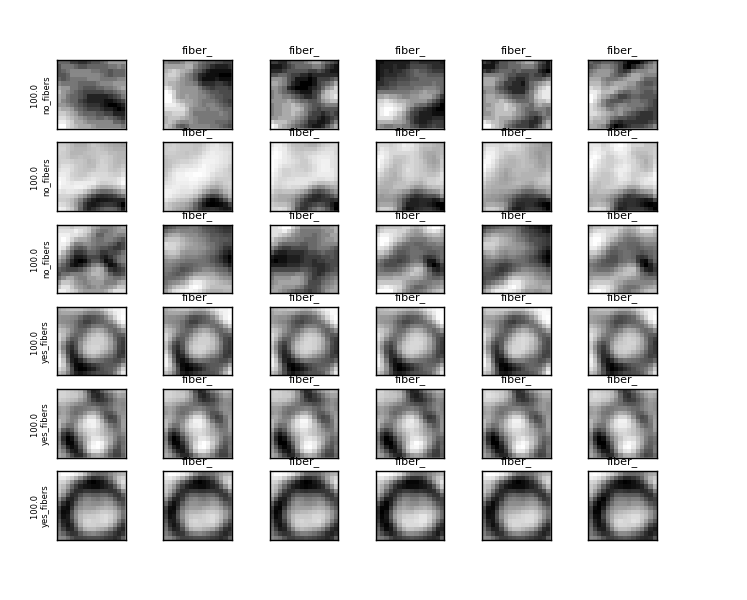
\includegraphics[width=2.5in]{img/flarom2.png}
\label{fig_second_case}}
\caption{Using TensorFlow: Dataset with more than three hundred thousand samples, used to train a deep
learning algorithm in order to separate fiber profiles (left) from other regions (right) as they
appear in micro tomography image from ceramic matrix composites. Accuracy results for this CNN are
99.788623\%, considering stratified training and tests sets, with 70\% and 30\% of the samples
respectively.}
\label{fig_sim}
\end{figure*}
%

\section{Results}

\subsection{Matconvnet}
A traditional Convolutional Neural Network (CNN) is parameterized by floating point weights and biases
and takes floating point data as input. In many cases, the floating point representation of these
parameters and input is more than necessary. The use of a more compact representation of the
parameters and input allows CNNs to be deployed on energy efficient architectures that operate with a
few bits and much lower memory footprint. This work focuses on data reduction and quantization schemes
that can be applied to a trained CNN for classifying scienti c simulation data. We show that each
neuron and synapse can be encoded with only one byte to maintain accuracy above 98\%.
\begin{figure}[h]
\centering
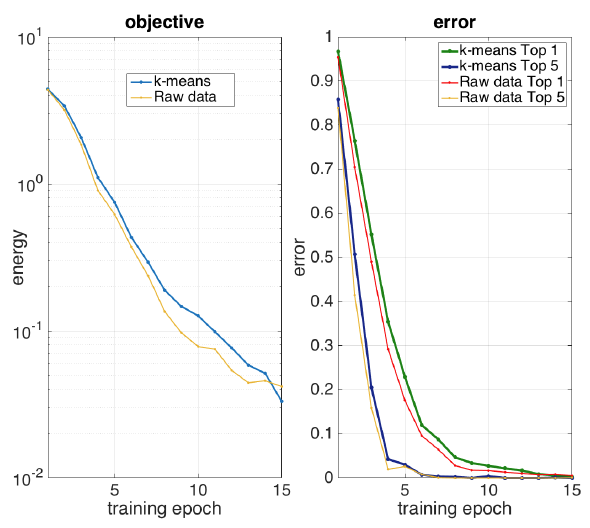
\includegraphics[width=\linewidth]{img/joao3.png}
\caption{Simulation results for the network.}
\label{fig_sim}
\end{figure}


\subsection{Neuromorphic computing}

\begin{figure}[h]
\centering
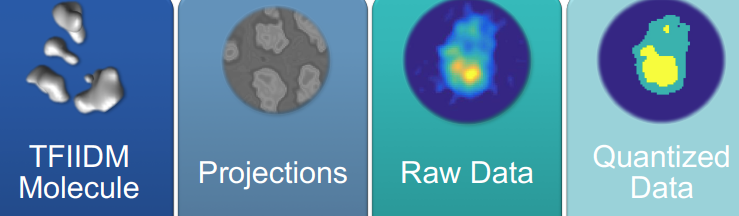
\includegraphics[width=\linewidth]{img/joao1.png}
\caption{Simulation results for the network.}
\label{fig_sim}
\end{figure}

\begin{figure}[h]
\centering
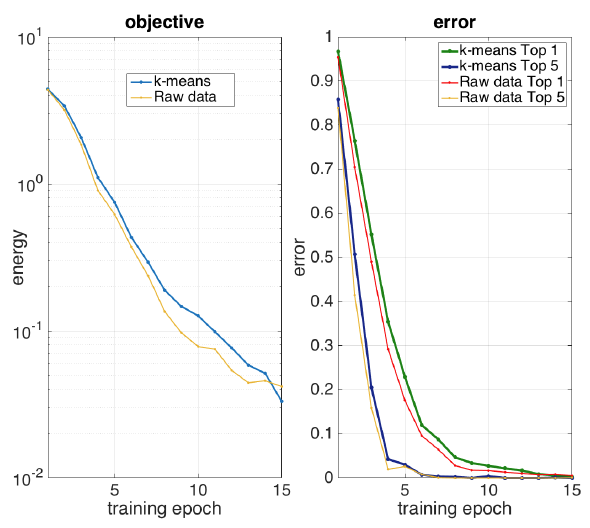
\includegraphics[width=\linewidth]{img/joao3.png}
\caption{Coisas do jao.}
\label{fig:cryem}
\end{figure}

IBM TN settings:
Corelet Programming Environment CPE Version 2.2.160518
CPE + tn-signal-processor to make a model
and run a model on the TrueNorth hardware
Matlab with MatConvNet

Fibers=216,650 samples
Non-fibers=105,120 samples
Each sample = 162 uint8 input (raw = no processing)
How: leverage curated data analyzed using sophisticated computer vision algorithms + user intervention

Preliminary results using the neuromorphic chip IBM TrueNorth
Specs and accuracy:
~3,200 cores < 1 chip = 4096 cores
Model = 
Train=70\%; test=30\%
Accuracy = 99.788623\%

What is next:
Interpret Eedn output results
Deploy TN on a testbed at NERSC
Port models to the chip at LBL
Evaluate on new samples coming from ALS

\subsection{NVIDIA DevBox}



\begin{figure*}[!t]
\centering
\subfloat[Case I]{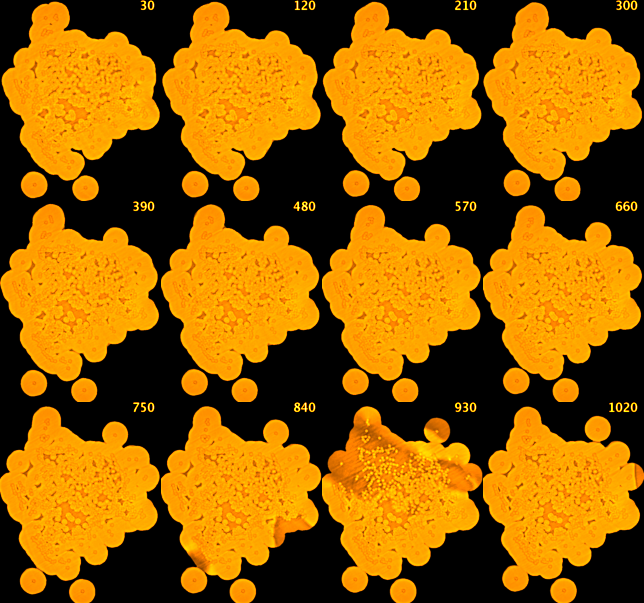
\includegraphics[width=.439\linewidth]{img/fiberMontage.png}
\label{fig_first_case}}
\hfil
\subfloat[Case II]{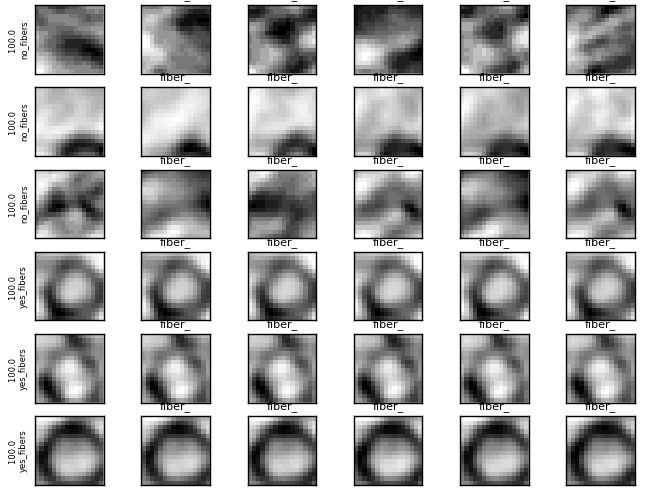
\includegraphics[width=.54\linewidth]{img/fiberCBIR.png}
\label{fig_second_case}}
\caption{Using TensorFlow: Dataset with more than three hundred thousand samples, used to train a deep
learning algorithm in order to separate fiber profiles (left) from other regions (right) as they
appear in micro tomography image from ceramic matrix composites. Accuracy results for this CNN are
99.788623\%, considering stratified training and tests sets, with 70\% and 30\% of the samples
respectively.}
\label{fig:pycbir}
\end{figure*}



\section{Conclusion}
The conclusion goes here.




% conference papers do not normally have an appendix


% use section* for acknowledgment
\section*{Acknowledgment}


The authors would like to thank...





% trigger a \newpage just before the given reference
% number - used to balance the columns on the last page
% adjust value as needed - may need to be readjusted if
% the document is modified later 
%\IEEEtriggeratref{8}
% The "triggered" command can be changed if desired:
%\IEEEtriggercmd{\enlargethispage{-5in}}

% references section

% can use a bibliography generated by BibTeX as a .bbl file
% BibTeX documentation can be easily obtained at:
% http://mirror.ctan.org/biblio/bibtex/contrib/doc/
% The IEEEtran BibTeX style support page is at:
% http://www.michaelshell.org/tex/ieeetran/bibtex/
%\bibliographystyle{IEEEtran}
% argument is your BibTeX string definitions and bibliography database(s)
%\bibliography{IEEEabrv,../bib/paper}
%
% <OR> manually copy in the resultant .bbl file
% set second argument of \begin to the number of references
% (used to reserve space for the reference number labels box)
\begin{thebibliography}{1}

\bibitem{IEEEhowto:kopka}
H.~Kopka and P.~W. Daly, \emph{A Guide to \LaTeX}, 3rd~ed.\hskip 1em plus
  0.5em minus 0.4em\relax Harlow, England: Addison-Wesley, 1999.

\end{thebibliography}




% that's all folks
\end{document}


